% Author Vahid Partovi Nia
% Copyright Huawei Technologies
% Network Mind Team



\documentclass[12pt]{beamer}

\usetheme{Hannover}
\setbeamercolor{section in sidebar shaded}{fg=black}

\usecolortheme{beaver}
\beamertemplatenavigationsymbolsempty

%  \usebeamertemplate{navigation symbols}\hfill
%  \insertframenumber{}/\inserttotalframenumber}
  

\useoutertheme{sidebar}
\pgfdeclareimage[width=2.5\baselineskip]{institut-logo}{fig/mcgill_logo}
\setbeamertemplate{footline}
{\raisebox{-2ex}{\pgfuseimage{institut-logo}}
%  \hfill
\hspace{5cm}
  \usebeamertemplate{navigation symbols}
  \insertframenumber{}/\inserttotalframenumber
  \hspace{3.8cm}
YCBS255
}
%\setbeamertemplate{sidebar right}{}
  
\setbeamercolor{block title}{fg=darkred}
\setbeamercolor{local structure}{fg=darkred}

\setbeamercolor{palette sidebar secondary}{fg=darkgray, bg=white}



\usefonttheme{professionalfonts} % using non standard fonts for beamer


\makeatletter
\beamer@nav@subsectionstyle{hide/hide/hide}
\makeatother

\titlegraphic{
\includegraphics[width=2cm]{fig/mcgill_logo}}




\usepackage{listings}
\usepackage{xcolor}
\def \y {\mathbf y}
\def \X {\mathbf X}
\def \A {\mathbf A}
\def \t {^\top}
\def \inv {^ {-1}}
\def \x {\mathbf x}
\def \bbeta {\boldsymbol \beta}
\def \eeps {\boldsymbol \varepsilon}
\def \TV {\mathrm{TV}}
\def \Radio {\mathrm{Radio}}
\def \Newspaper {\mathrm{Newspaper}}
\def \Sales {\mathrm{Sales}}
\def \Balance {\mathrm{Balance}}
\def \Default {\mathrm{Default}}

\definecolor{capri}{rgb}{0.0, 0.75, 1.0}
\definecolor{darkcyan}{rgb}{0.0, 0.55, 0.55}
\definecolor{deepfuchsia}{rgb}{0.76, 0.33, 0.76}
\begin{document}

% no title and no author on sidebar
\title[]{Cross-validation}   
\author[]{Vahid Partovi Nia} 
\institute{Lecture 04}
\date{13 November 2018}


\makeatletter
  \begin{frame}[plain]
    \hspace*{-\beamer@leftsidebar}%
    \advance\textwidth by \beamer@leftsidebar\relax
    \beamer@leftsidebar=\z@
    \begin{minipage}{\textwidth}\par%
      \maketitle
    \end{minipage}
  \end{frame}
  \makeatother



\frame{\frametitle{Outline}\tableofcontents} 

\setbeamertemplate{sidebar left}[sidebar theme]


\section{Flexibility}




\frame{\frametitle{statsmodels}
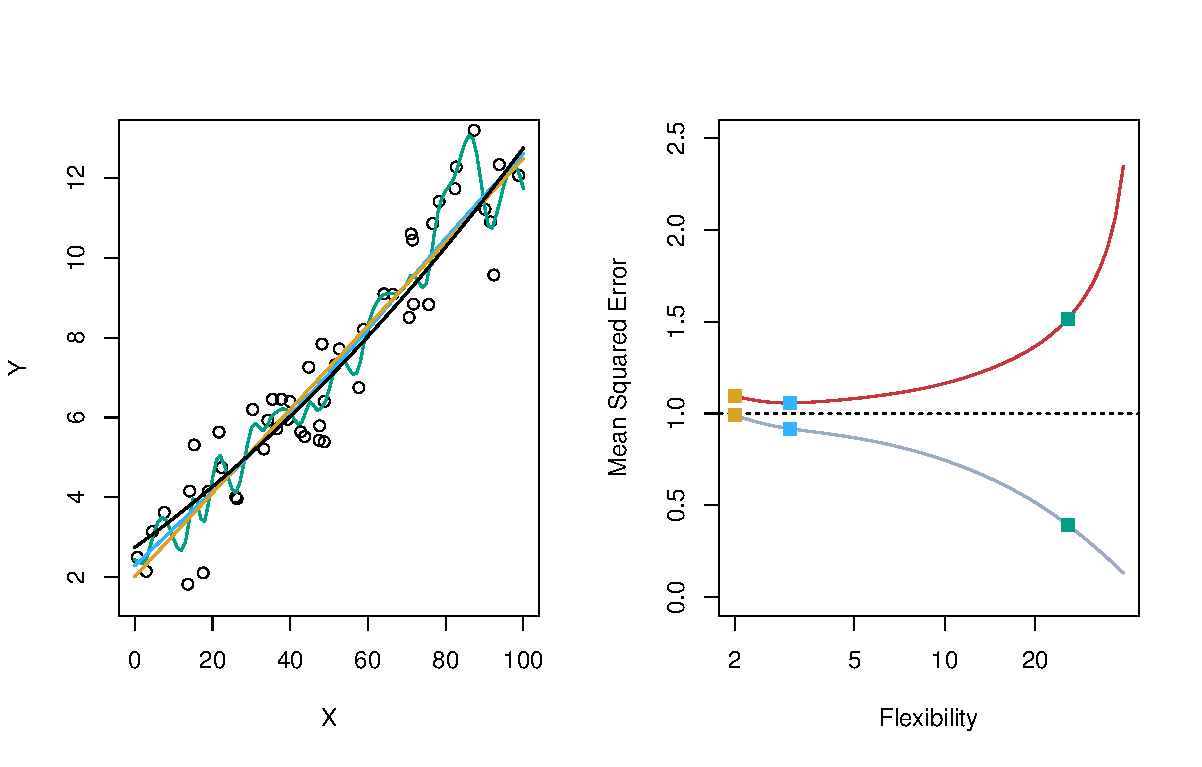
\includegraphics[width=\textwidth]{fig/2-10}
}

\frame{\frametitle{statsmodels}
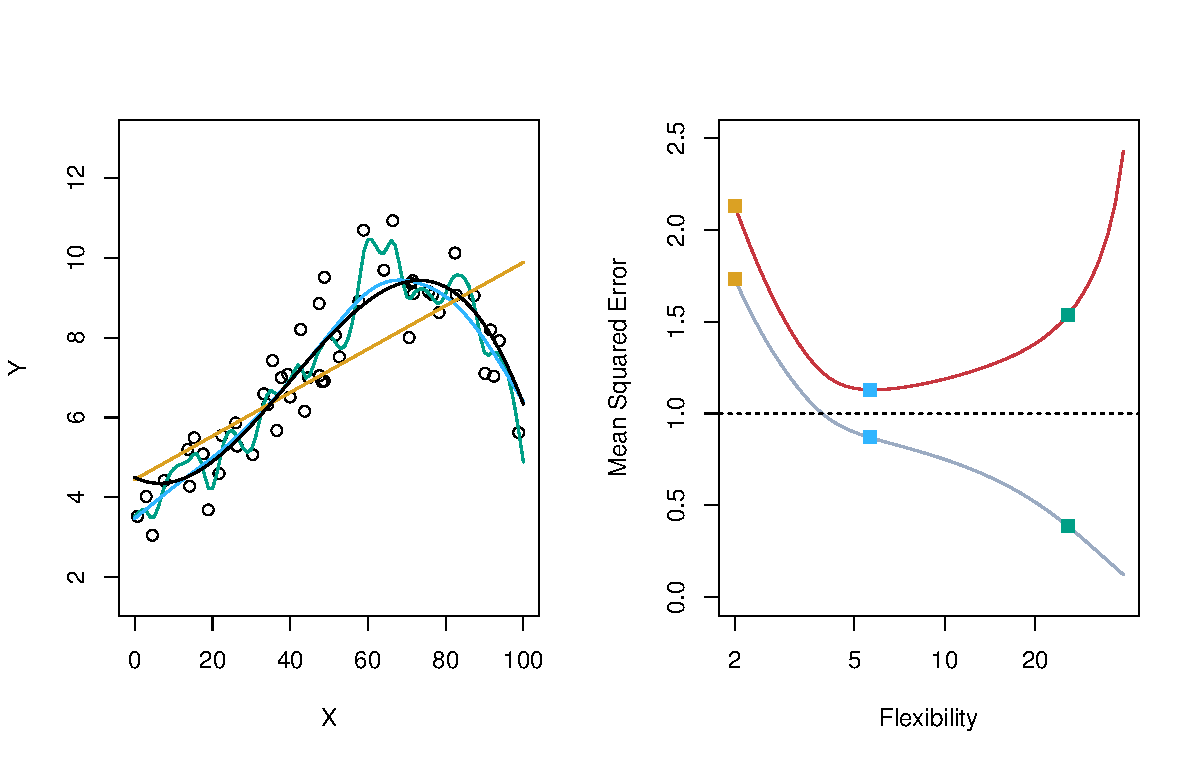
\includegraphics[width=\textwidth]{fig/2-9}
}

\frame{\frametitle{Auto Dataset}
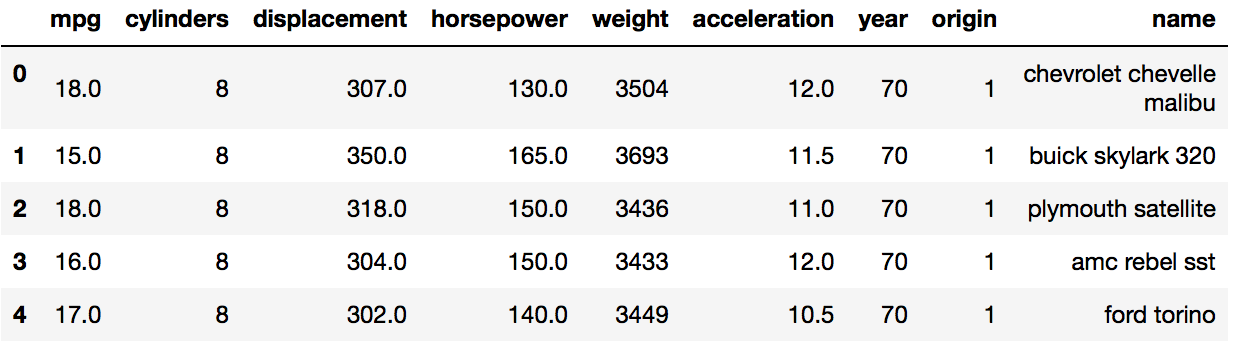
\includegraphics[width=\textwidth]{fig/autodata}
}

\begin{frame}[fragile]
\tiny
\begin{lstlisting}
import pandas as pd
path='data/'
filename = path+'Auto.csv'
auto = pd.read_csv(filename, na_values=['?'], na_filter=True)
auto = auto.dropna()
\end{lstlisting} 
\pause
\begin{lstlisting}
import matplotlib.pyplot as plt
%matplotlib inline
plt.plot(auto['horsepower'], auto['mpg'], 'or', mfc='none');
\end{lstlisting} 
\pause

\begin{lstlisting}
import seaborn as sns           
sns.regplot(x="horsepower", y="mpg", data=auto, ci=False,
    scatter_kws={"color":"r", "alpha":0.3, "s":100},
    line_kws={"color":"b", "alpha":0.5, "lw":4}, marker="o", order=2)
    \end{lstlisting} 
\end{frame}

\frame{
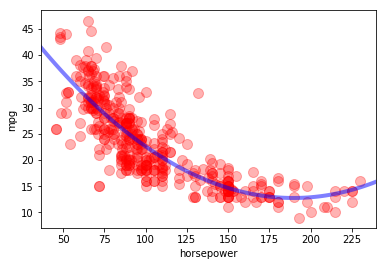
\includegraphics[width=\textwidth]{fig/regplot}
}

\section{Model Selection}

\begin{frame}[fragile]
\tiny
\begin{lstlisting}
import numpy as np
import statsmodels.formula.api as smf
model = smf.ols(formula='mpg ~ horsepower', data=auto)

lr1 = model.fit()
lr1.summary2()

lr1.aic 
\end{lstlisting}
\end{frame}


\begin{frame}[fragile]
\tiny
\begin{lstlisting}
model = smf.ols(formula='mpg ~ horsepower +
                np.power(horsepower,2)', data = auto)
lr2 = model.fit()
lr2.aic
\end{lstlisting}
\pause
\begin{lstlisting}
model = smf.ols(formula='mpg ~ horsepower +
		np.power(horsepower,2)+ np.power(horsepower,3)',
		data = auto)
lr3 = model.fit()
lr3.aic
\end{lstlisting}
\end{frame}


\section{Cross-validation}

\frame{\frametitle{Leave-one-out}
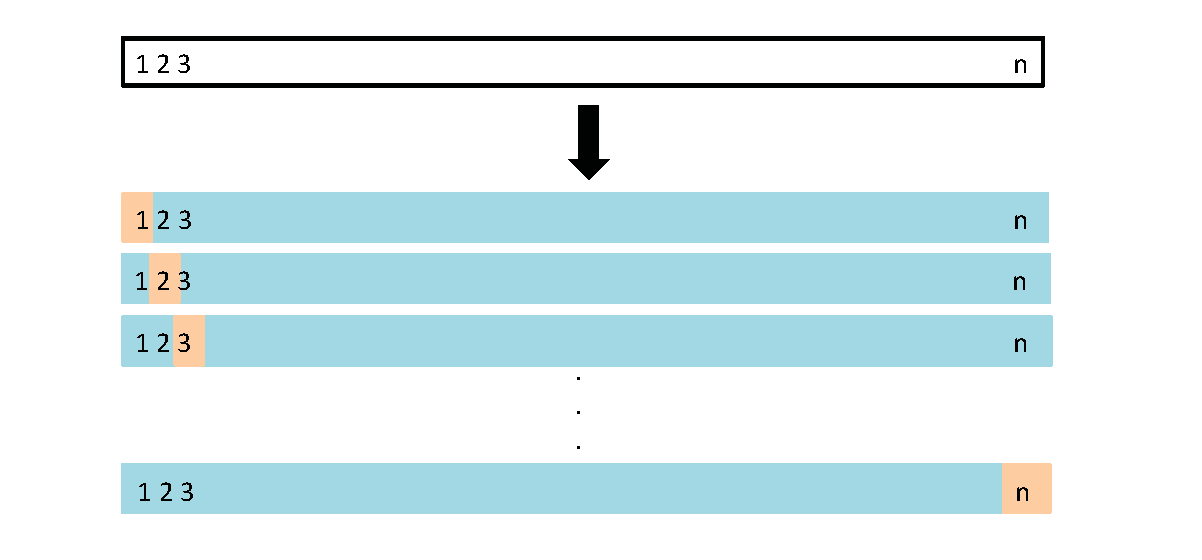
\includegraphics[width=\textwidth]{fig/5-3}
$$\mathrm{RSS}= n \hat \sigma^2 =\sum_{i=1}^n ( {\color{orange}y_i} - {\color{orange}\hat y_i})^2 $$
}


\begin{frame}[fragile]
\tiny
\begin{lstlisting}
from sklearn.model_selection import LeaveOneOut
from sklearn.linear_model import LinearRegression
loo = LeaveOneOut()
loo.get_n_splits(auto)
\end{lstlisting}
\begin{lstlisting}
\end{lstlisting}
\end{frame}


\begin{frame}[fragile]
\tiny
\begin{lstlisting}
X = auto[['horsepower']].values
y = auto['mpg'].values

rss = np.zeros(auto.shape[0])
i = 0
for train_i, test_i in loo.split(auto):
    lr = LinearRegression() 
    lr = lr.fit(X[train_i], y[train_i])
    rss[i]=(lr.predict(X[test_i]) - y[test_i])**2
    i += 1
np.sum(rss)\end{lstlisting}
\end{frame}

\begin{frame}[fragile]
\tiny
\begin{lstlisting}
X = auto[['horsepower', 'displacement']].values
rss = np.zeros(auto.shape[0])
i = 0
for train_i, test_i in loo.split(auto):
    lr = LinearRegression() 
    lr = lr.fit(X[train_i], y[train_i])
    rss[i]=(lr.predict(X[test_i]) - y[test_i])**2
    i += 1
np.sum(rss)
\end{lstlisting}
\end{frame}


\frame{\frametitle{$5$-fold}
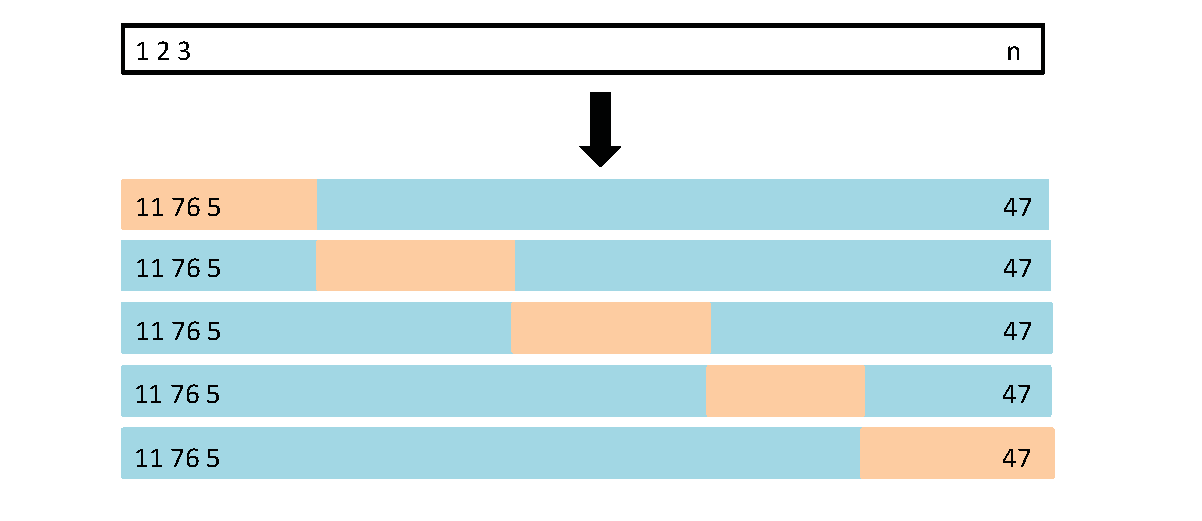
\includegraphics[width=0.9\textwidth]{fig/5-5}\\
$\mathrm{RSS} =  \left\{\mathrm{RSS}_1 + \cdots + \mathrm{RSS}_5\right\}$
 {\tiny
\begin{eqnarray*}
\mathrm{RSS_1} &=&  \sum_{i=1}^{n/5} ( {\color{orange}y_i} - {\color{orange}\hat y_i})^2 \\
\mathrm{RSS_2} &=&  \sum_{i=1}^{n/5} ( {\color{orange}y_i} - {\color{orange}\hat y_i})^2 \\
&\vdots& \\
\mathrm{RSS_5} &=&  \sum_{i=1}^{n/5} ( {\color{orange}y_i} - {\color{orange}\hat y_i})^2 \\
\end{eqnarray*}
}
}


\begin{frame}[fragile]\frametitle{5-fold}
\tiny
\begin{lstlisting}
from sklearn.model_selection import KFold
X = auto[['horsepower', 'displacement']].values
k = 5
rss = np.zeros(k)
kf = KFold(n_splits=k, shuffle=True)
i = 0
for train_i, test_i in kf.split(auto):
    lr = LinearRegression() 
    lr = lr.fit(X[train_i], y[train_i])
    rss[i]=np.sum((lr.predict(X[test_i]) - y[test_i])**2)
    i+=1
rss
\end{lstlisting}
\end{frame}

\begin{frame}[fragile]
Implement 10-fold
\end{frame}




%\begin{frame}[fragile]
%\begin{lstlisting}
%\end{lstlisting}
%\end{frame}


%\begin{lstlisting}
%\end{lstlisting} 

%\frame{\frametitle{}
%\includegraphics[width=0.5\textwidth]{fig/}
%}
%\frame{\frametitle{}
%\includegraphics[width=0.5\textwidth]{fig/}
%}
%\frame{\frametitle{}
%\includegraphics[width=0.5\textwidth]{fig/}
%}
%\frame{\frametitle{}
%\includegraphics[width=0.5\textwidth]{fig/}
%}
%\frame{\frametitle{}
%\includegraphics[width=0.5\textwidth]{fig/}
%}
%
%
%
%

\end{document}
